\documentclass[aspectratio=169]{beamer}

% ---------- ENCODING & FONTS ----------
\usepackage[utf8]{inputenc}
\usepackage[T1]{fontenc}

% ---------- THEME & LOOK ----------
\usetheme{Madrid}
\usecolortheme{seahorse}
\usefonttheme{professionalfonts}
\setbeamertemplate{navigation symbols}{}
\setbeamercovered{transparent}
\setbeamertemplate{itemize items}[circle]
\setbeamertemplate{enumerate items}[default]
\setlength{\parskip}{0.25em}

% ---------- COLORS ----------
% Beamer already loads xcolor, so we just define our colors
\definecolor{accent}{RGB}{0,92,184}
\definecolor{soft}{RGB}{233,244,255}
\definecolor{lightred}{RGB}{245,210,210}
\setbeamercolor{structure}{fg=accent}
\setbeamercolor{title}{fg=white,bg=accent}
\setbeamercolor{frametitle}{fg=accent}
\setbeamercolor{block title}{bg=accent!12,fg=accent}
\setbeamercolor{block body}{bg=soft}

% ---------- PACKAGES ----------
\usepackage{booktabs}
\usepackage{amsmath, amssymb}
\usepackage{array}
\usepackage{multirow}
\usepackage{hyperref}
\hypersetup{colorlinks=true,linkcolor=accent,urlcolor=accent}

% ---------- SAFE TRANSITION FALLBACK ----------
\makeatletter
\@ifundefined{transfade}{\newcommand{\transfade}[1][]{}}{}
\makeatother

% ---------- PLACEHOLDER BOX FOR FIGURES ----------
\newcommand{\placeholderbox}[2][0.82\linewidth]{%
  \begin{center}
    \fbox{\begin{minipage}[c][0.46\textheight][c]{#1}
      \centering \vspace{0.3em}
      \textbf{#2}\\[0.6em]
      \emph{Insert figure/diagram here later.}
    \end{minipage}}
  \end{center}
}

% ---------- TITLE ----------
\title{\textbf{Fiscal Policy \vspace{.5cm}\\  }}
\subtitle{ {\large ECON 101 - Macroeconomics}}
%\institute{UNBC}
\author{Muhebullah Karimzada}
\date{Winter 2026}



\begin{document}

% ============================================================
% TITLE
% ============================================================
\begin{frame}[plain]
  \titlepage
\end{frame}

% ============================================================
\begin{frame}{Chapter Outline}
\transfade
\begin{itemize}
  \item \textbf{12.1} What is Fiscal Policy?
  \item \textbf{12.2} The Effects of Fiscal Policy on Real GDP and the Price Level
  \item \textbf{12.4} Government Purchases and Tax Multipliers
  \item \textbf{12.5} The Limits of Fiscal Policy as a Stimulus
  \item \textbf{12.6} Deficits, Surpluses, and Federal Government Debt
  \item \textbf{12.7} The Effects of Fiscal Policy in the Long Run
  \item \textbf{Appendix} A Closer Look at the Multiplier
\end{itemize}
\end{frame}

% ============================================================
\section{12.1 What is Fiscal Policy?}
% ============================================================

\begin{frame}{12.1 Learning Objective}
\transfade
\begin{block}{Goal}
Define fiscal policy.
\end{block}
\begin{itemize}
  \item Understand what economists mean by \textbf{fiscal policy}.
  \item Distinguish between:
  \begin{itemize}
    \item automatic stabilizers, and
    \item discretionary fiscal policy.
  \end{itemize}
  \item Connect fiscal policy to real-world Canadian examples (EI, tax changes, infrastructure spending).
\end{itemize}
\end{frame}

\begin{frame}{What is Fiscal Policy?}
\transfade
\begin{itemize}
  \item \textbf{Fiscal policy} refers to changes in \alert{federal taxes and purchases}
        that are intended to achieve \textbf{macroeconomic policy objectives}.
  \item Provincial and territorial taxes and spending:
  \begin{itemize}
    \item are important,
    \item but are not generally aimed at affecting \emph{national}-level macro goals in the same direct way.
  \end{itemize}
  \item The key idea:
  \begin{itemize}
    \item the federal government can \emph{shift aggregate demand} by changing its spending and tax decisions.
  \end{itemize}
\end{itemize}
\end{frame}

\begin{frame}{Automatic Stabilizers vs. Discretionary Policy}
\transfade
\begin{itemize}
  \item Some forms of government spending and taxes automatically move with the business cycle:
  \begin{block}{Automatic stabilizers}
    Government spending and taxes that \alert{automatically increase or decrease}
    with the business cycle, without any new legislation.
  \end{block}
  \item Example:
  \begin{itemize}
    \item Employment Insurance (EI) payments rise in a recession:
    \item more people become unemployed and qualify for benefits.
  \end{itemize}
  \item \textbf{Discretionary fiscal policy}:
  \begin{itemize}
    \item intentional actions the government takes to change spending or taxes,
    \item e.g. a new infrastructure program, or a legislated cut in the GST.
  \end{itemize}
\end{itemize}
\end{frame}

% ============================================================
\section{12.2 Effects of Fiscal Policy on GDP and the Price Level}
% ============================================================

\begin{frame}{12.2 Learning Objective}
\transfade
\begin{block}{Goal}
Explain how fiscal policy affects aggregate demand and how the government can use fiscal policy to stabilize the economy.
\end{block}
\begin{itemize}
  \item The government carries out fiscal policy through:
  \begin{itemize}
    \item changes in \textbf{government purchases} (\(G\)),
    \item changes in \textbf{taxes} (\(T\)).
  \end{itemize}
  \item A change in \(G\) affects aggregate demand \alert{directly}.
  \item A change in \(T\) affects income and consumption, and so affects aggregate demand \alert{indirectly}.
\end{itemize}
\end{frame}

\begin{frame}{Expansionary vs. Contractionary Fiscal Policy}
\transfade
\begin{itemize}
  \item \textbf{Expansionary fiscal policy}:
  \begin{itemize}
    \item increasing government purchases, or
    \item decreasing taxes.
  \end{itemize}
  \item \textbf{Contractionary fiscal policy}:
  \begin{itemize}
    \item decreasing government purchases, or
    \item increasing taxes.
  \end{itemize}
  \item Both types work through the aggregate demand channel:
  \begin{itemize}
    \item higher \(G\) and lower \(T\) shift AD \textbf{right},
    \item lower \(G\) and higher \(T\) shift AD \textbf{left}.
  \end{itemize}
\end{itemize}
\end{frame}

\begin{frame}{Figure 12.7 -- Fiscal Policy (1 of 2) }
\centering
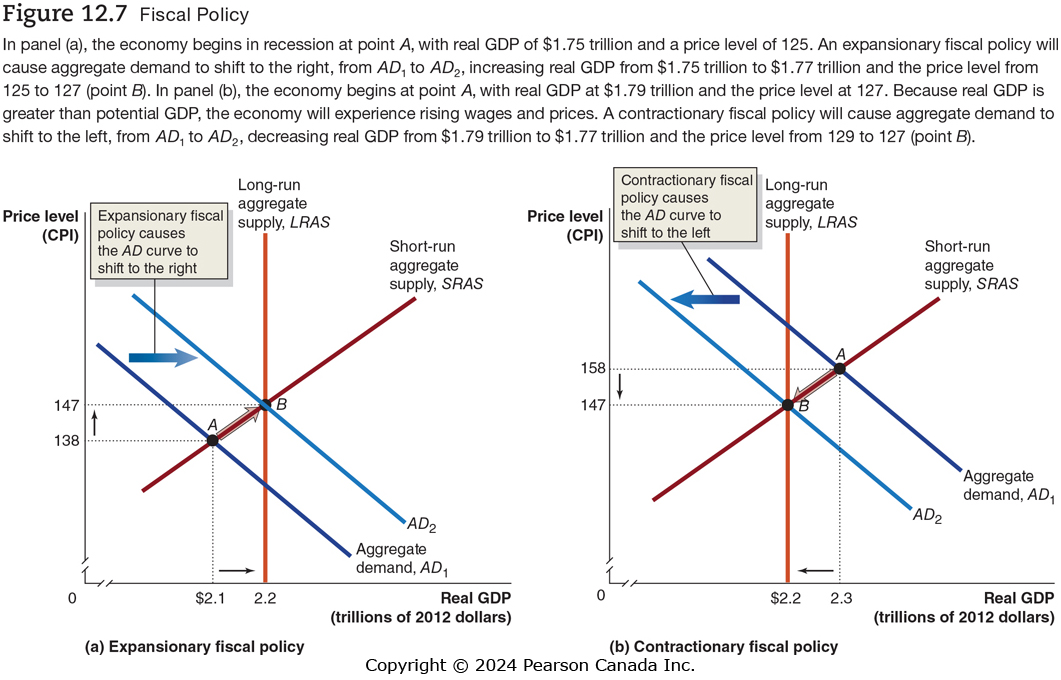
\includegraphics[width=0.7\linewidth]{Fig12-007}
\end{frame}

\begin{frame}{Expansionary Fiscal Policy}
\transfade
\begin{itemize}
  \item \textbf{Expansionary fiscal policy} involves:
  \begin{itemize}
    \item increasing government purchases, or
    \item decreasing taxes.
  \end{itemize}
  \item If the government believes real GDP will be \alert{below potential GDP}:
  \begin{itemize}
    \item it can enact expansionary fiscal policy to close the \textbf{recessionary gap}.
  \end{itemize}
  \item Effects:
  \begin{itemize}
    \item AD shifts right,
    \item real GDP and employment rise,
    \item the price level also rises relative to what it otherwise would have been.
  \end{itemize}
\end{itemize}
\end{frame}

\begin{frame}{Figure 12.7 -- Fiscal Policy (2 of 2) }
\centering
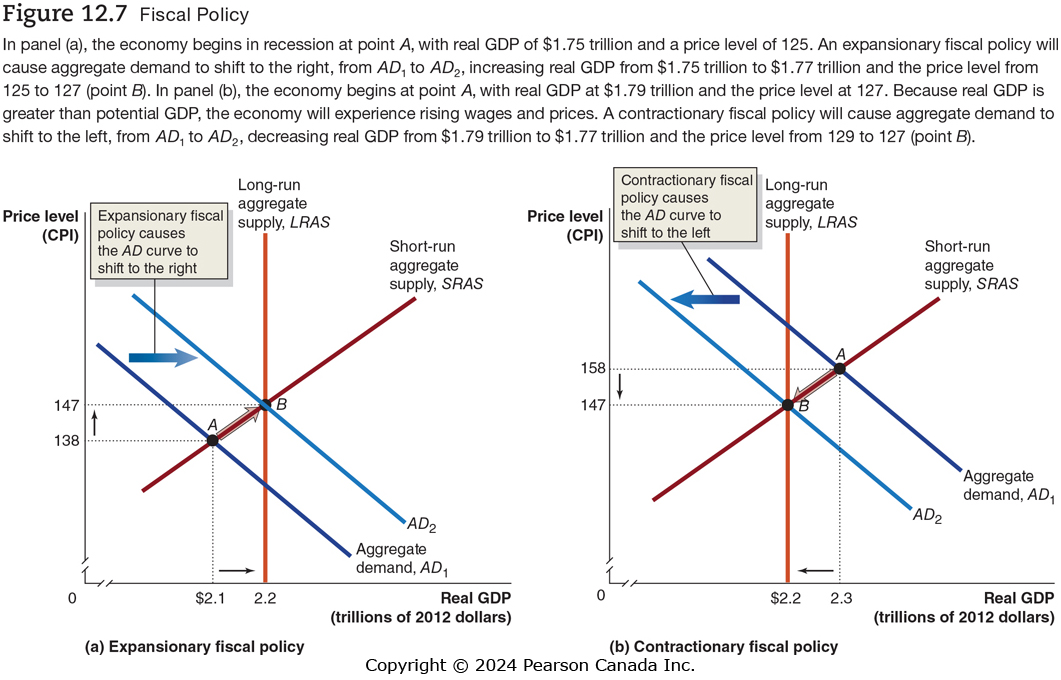
\includegraphics[width=0.7\linewidth]{Fig12-007}
\end{frame}

\begin{frame}{Contractionary Fiscal Policy}
\transfade
\begin{itemize}
  \item \textbf{Contractionary fiscal policy} involves:
  \begin{itemize}
    \item decreasing government purchases, or
    \item increasing taxes.
  \end{itemize}
  \item If the government believes real GDP will be \alert{above potential GDP}:
  \begin{itemize}
    \item it can enact contractionary policy to reduce inflationary pressure.
  \end{itemize}
  \item Effects:
  \begin{itemize}
    \item AD shifts left,
    \item real GDP and inflation both decrease relative to what they otherwise would have been.
  \end{itemize}
\end{itemize}
\end{frame}

\begin{frame}{Table 12.1 Countercyclical Fiscal Policy}
\transfade
\begin{center}
\small
\begin{tabular}{p{0.19\linewidth} p{0.19\linewidth} p{0.32\linewidth} p{0.22\linewidth}}
\toprule
\textbf{Problem} &
\textbf{Type of Policy Required} &
\textbf{Actions by Congress and the President} &
\textbf{Result} \\
\midrule
Recession &
Expansionary &
Increase government purchases or cut taxes &
Real GDP and the price level rise. \\
Rising inflation &
Contractionary &
Decrease government purchases or raise taxes &
Real GDP and the price level fall. \\
\bottomrule
\end{tabular}
\end{center}
\end{frame}


\begin{frame}{Interpreting Table 12.1}
\transfade
\begin{itemize}
  \item The table summarizes \textbf{countercyclical} fiscal policy:
  \begin{itemize}
    \item policy that moves the economy in the opposite direction of the business cycle.
  \end{itemize}
  \item Bear in mind:
  \begin{itemize}
    \item These effects are described \textbf{ceteris paribus}:
    \item everything else (including monetary policy) is assumed unchanged.
  \end{itemize}
  \item Contractionary fiscal policy is not literally making prices fall:
  \begin{itemize}
    \item it is keeping inflation \alert{lower than it otherwise would have been}.
  \end{itemize}
\end{itemize}
\end{frame}

% ============================================================
\section{12.4 Government Purchases and Tax Multipliers}
% ============================================================

\begin{frame}{12.4 Learning Objective}
\transfade
\begin{block}{Goal}
Explain how the government purchases and tax multipliers work.
\end{block}
\begin{itemize}
  \item An initial change in \(G\) or \(T\) sets off:
  \begin{itemize}
    \item an \textbf{autonomous} change in spending, and
    \item a chain of \textbf{induced} changes via consumption.
  \end{itemize}
  \item Together these create a \textbf{multiplier effect} on real GDP.
\end{itemize}
\end{frame}

\begin{frame}{Autonomous vs. Induced Effects and the Multiplier}
\transfade
\begin{itemize}
  \item If the government increases spending on goods and services:
  \begin{itemize}
    \item AD increases immediately – this is the \textbf{autonomous} increase.
  \end{itemize}
  \item People receiving this extra spending see their income rise:
  \begin{itemize}
    \item they increase consumption spending,
    \item which further raises AD – this is the \textbf{induced} increase.
  \end{itemize}
  \item The series of induced increases in consumption spending that results from the initial increase in autonomous expenditures is the:
  \begin{block}{Multiplier effect}
    The process where an initial change in autonomous spending leads to a larger change in equilibrium real GDP.
  \end{block}
\end{itemize}
\end{frame}

\begin{frame}{Figure 12.10 -- The Multiplier Effect and AD }
\centering
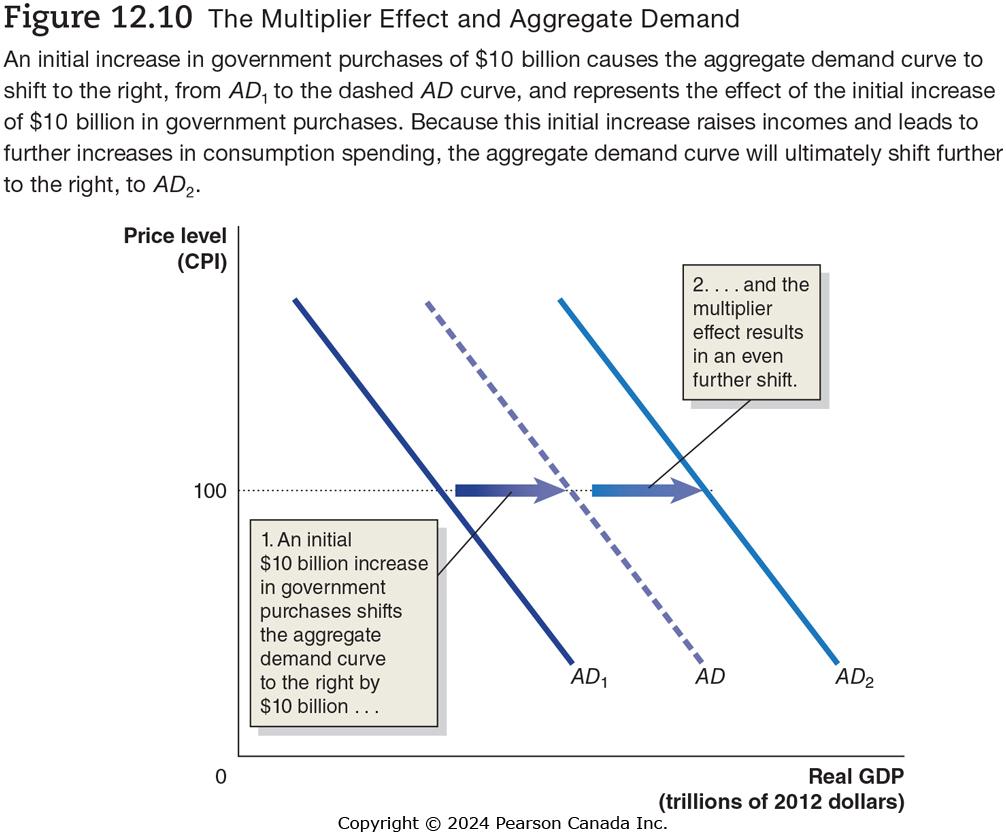
\includegraphics[width=0.56\linewidth]{Fig12-010}
\end{frame}

\begin{frame}{Figure 12.11 -- Example: \texorpdfstring{\$10}{\$10} Billion Increase in \(G\)}
\centering
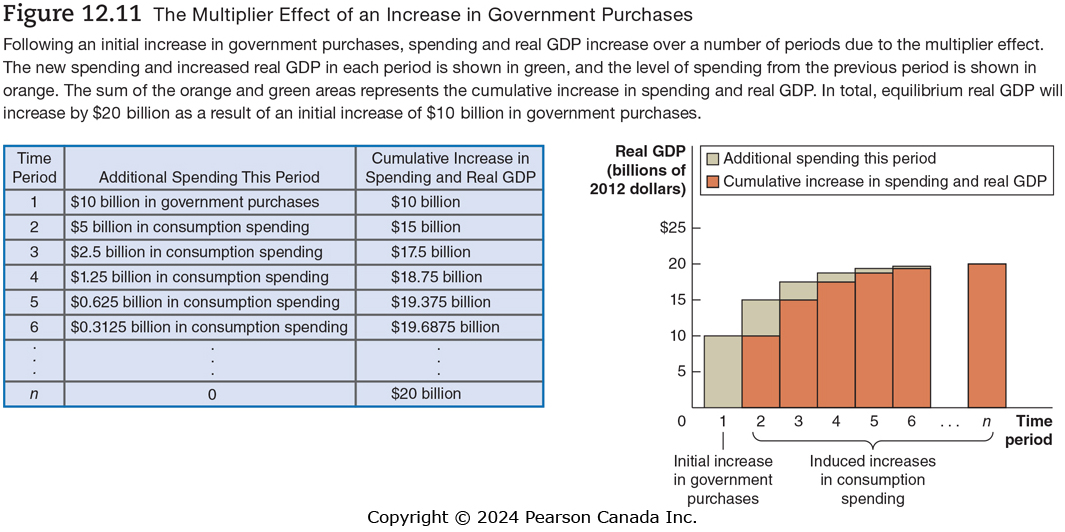
\includegraphics[width=0.9\linewidth]{Fig12-011}
\end{frame}

\begin{frame}{Numerical Example of the Multiplier}
\transfade
\begin{itemize}
  \item Suppose each increase in spending induces an increase in consumption equal to one-half of the increase in income:
  \begin{itemize}
    \item that is, the marginal propensity to consume (MPC) on domestic goods is \(0.5\).
  \end{itemize}
  \item A \$10 billion increase in government purchases:
  \begin{itemize}
    \item initially raises AD by \$10 billion (autonomous),
    \item then induces an additional \$5 billion in new consumption,
    \item then another \$2.5 billion, and so on.
  \end{itemize}
  \item Over time, the total increase in real GDP is \textbf{larger} than the initial \$10 billion increase in \(G\).
\end{itemize}
\end{frame}

\begin{frame}{Multipliers for Government Purchases and Taxes}
\transfade
\begin{itemize}
  \item We describe the total effect of a change in \(G\) or \(T\) by the change in equilibrium real GDP:
  \begin{itemize}
    \item \textbf{Government purchases multiplier}:
      \[
        \frac{\Delta Y}{\Delta G}
      \]
    \item \textbf{Tax multiplier}:
      \[
        \frac{\Delta Y}{\Delta T}
      \]
  \end{itemize}
  \item The tax multiplier is \textbf{negative}:
  \begin{itemize}
    \item an increase in taxes decreases equilibrium real GDP,
    \item a decrease in taxes increases equilibrium real GDP.
  \end{itemize}
  \item The tax multiplier is \textbf{smaller in absolute value} than the government purchases multiplier, because a tax cut is partially \emph{saved} and partially \emph{spent}.
\end{itemize}
\end{frame}

\begin{frame}{Changes in Tax Rates}
\transfade
\begin{itemize}
  \item The tax multiplier above applies to changes in the \textbf{amount} of taxes, holding tax rates fixed.
  \item Decreases in \textbf{tax rates} have a slightly different effect:
  \begin{itemize}
    \item increase the disposable income of households,
    \item increase their consumption spending,
    \item increase the size of the multiplier effect, because more of any income change shows up as disposable income.
  \end{itemize}
\end{itemize}
\end{frame}

\begin{frame}{Figure 12.12 -- Multiplier and AS }
\centering
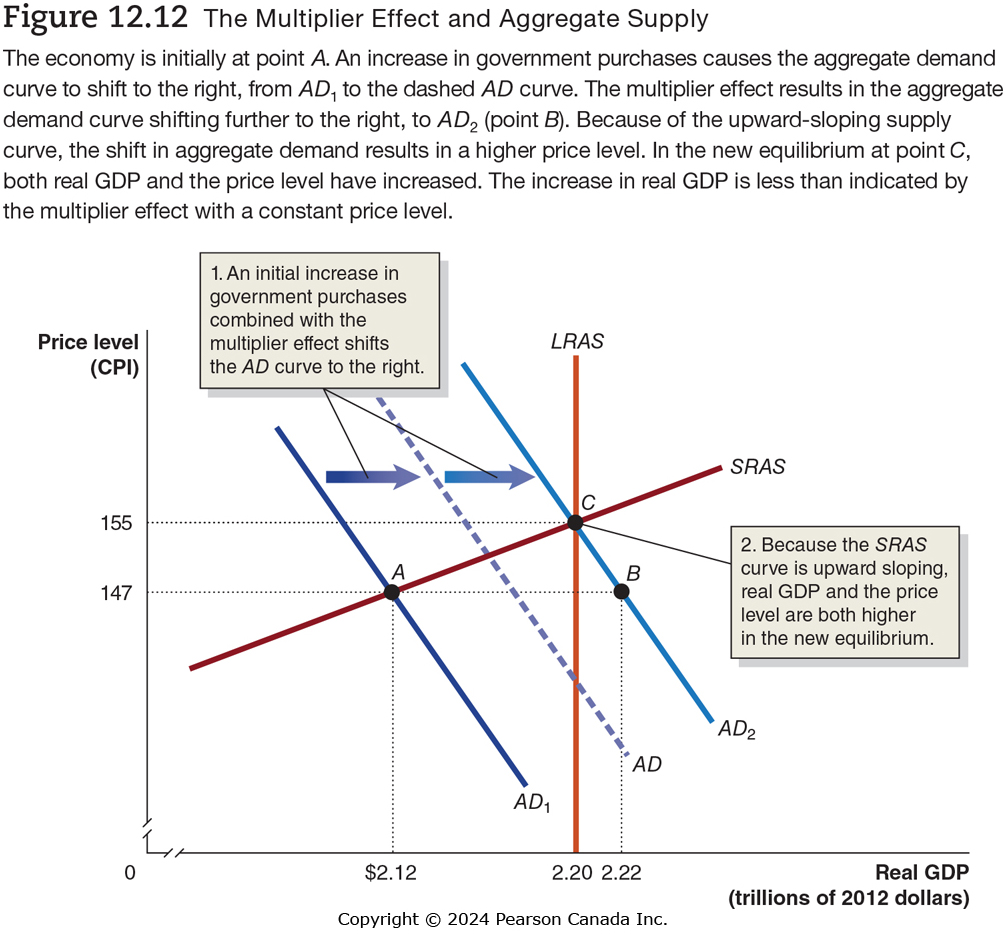
\includegraphics[width=0.5\linewidth]{Fig12-012}
\end{frame}

\begin{frame}{Multipliers with an Upward-Sloping SRAS}
\transfade
\begin{itemize}
  \item With an upward-sloping short-run aggregate supply (SRAS) curve:
  \begin{itemize}
    \item an increase in AD raises \textbf{both} real GDP and the price level.
  \end{itemize}
  \item Example:
  \begin{itemize}
    \item suppose autonomous and induced effects increase AD by \$100 billion.
    \item Real GDP might increase from \$2{,}120 billion to \$2{,}220 billion,
    \item while the price level also rises.
  \end{itemize}
  \item So part of the multiplier “shows up” as higher prices, not just higher real output.
\end{itemize}
\end{frame}

\begin{frame}{Multipliers Work in Both Directions}
\transfade
\begin{itemize}
  \item An \alert{increase} in government purchases and a \alert{cut} in taxes have a \textbf{positive} multiplier effect.
  \item A \alert{decrease} in government purchases and an \alert{increase} in taxes have a \textbf{negative} multiplier effect.
  \item Example:
  \begin{itemize}
    \item a reduction in government spending on infrastructure initially affects contractors,
    \item then suppliers and employees of those contractors,
    \item then other firms and workers,
    \item leading to a multiplied reduction in real GDP.
  \end{itemize}
\end{itemize}
\end{frame}

% ============================================================
\section{12.5 The Limits of Fiscal Policy as a Stimulus}
% ============================================================

\begin{frame}{12.5 Learning Objective}
\transfade
\begin{block}{Goal}
Discuss the difficulties that can arise in implementing fiscal policy.
\end{block}
\begin{itemize}
  \item Fiscal policy is powerful in theory but may be less effective in practice.
  \item Key issues:
  \begin{itemize}
    \item timing and lags,
    \item crowding out of private spending.
  \end{itemize}
\end{itemize}
\end{frame}

\begin{frame}{Timing Problems}
\transfade
\begin{itemize}
  \item Fiscal policy suffers from significant delays:
  \begin{enumerate}
    \item \textbf{Legislative delay}
      \begin{itemize}
        \item Parliament must debate and agree on changes to spending or taxes.
      \end{itemize}
    \item \textbf{Implementation delay}
      \begin{itemize}
        \item Large spending projects (e.g. infrastructure) may take months or years to actually begin, even after approval.
      \end{itemize}
  \end{enumerate}
  \item Because of these delays, fiscal stimulus may hit the economy:
  \begin{itemize}
    \item after the recession is already ending,
    \item potentially making the next boom and bust worse.
  \end{itemize}
\end{itemize}
\end{frame}

\begin{frame}{Crowding Out}
\transfade
\begin{block}{Crowding out}
A decline in private expenditures (consumption, investment, or net exports)
as a result of an increase in government purchases.
\end{block}
\begin{itemize}
  \item When the government increases spending, it often finances this by issuing bonds.
  \item Higher government borrowing can:
  \begin{itemize}
    \item increase the demand for money and credit,
    \item push up interest rates,
    \item reduce private investment, consumption, and net exports.
  \end{itemize}
\end{itemize}
\end{frame}

\begin{frame}{Figure 12.13 -- Expansionary Fiscal Policy and Interest Rates }
\centering
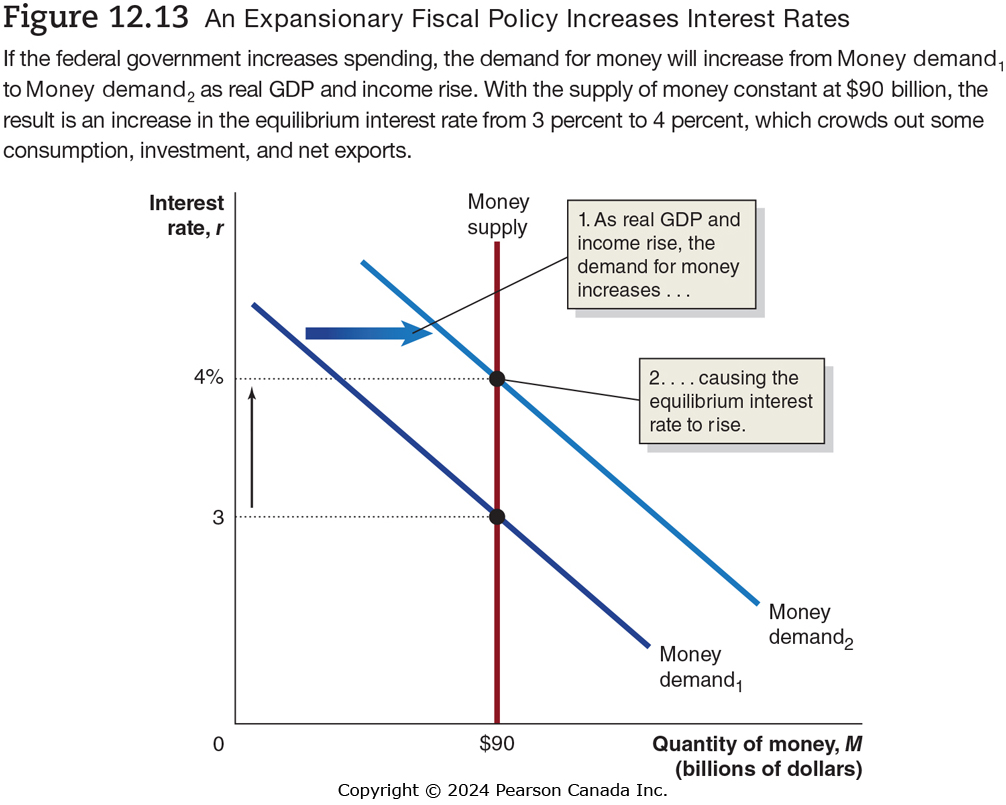
\includegraphics[width=0.57\linewidth]{Fig12-013}
\end{frame}

\begin{frame}{Figure 12.14 -- Crowding Out in the Short Run}
\centering
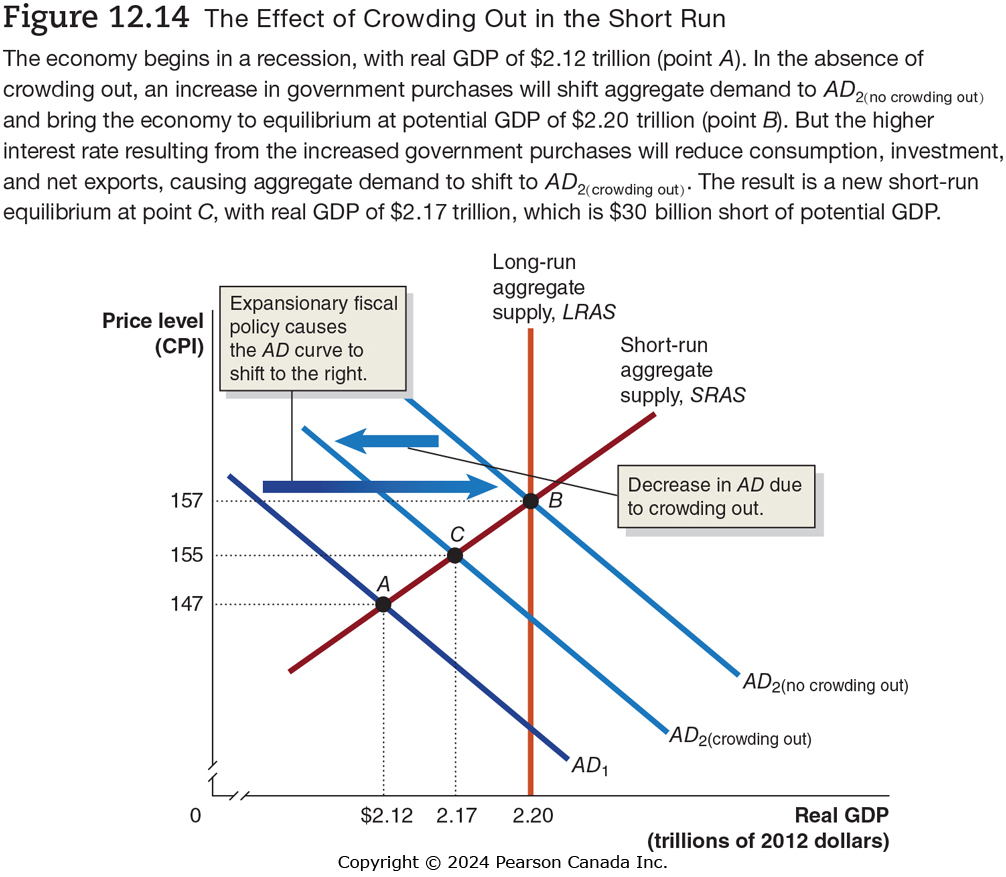
\includegraphics[width=0.57\linewidth]{Fig12-014}
\end{frame}

\begin{frame}{Crowding Out: Short Run vs. Long Run}
\transfade
\begin{itemize}
  \item In the \textbf{short run}:
  \begin{itemize}
    \item an increase in \(G\) raises AD,
    \item but higher interest rates partly offset this via lower C, I, and NX.
  \end{itemize}
  \item In the \textbf{long run}:
  \begin{itemize}
    \item the economy returns to potential GDP,
    \item the reduction in private spending ultimately \textbf{exactly offsets} the increase in government purchases,
    \item so real GDP is unchanged compared to potential.
  \end{itemize}
\end{itemize}
\end{frame}

% ============================================================
\section{12.6 Deficits, Surpluses, and Federal Government Debt}
% ============================================================

\begin{frame}{12.6 Learning Objective}
\transfade
\begin{block}{Goal}
Define federal budget deficit and federal government debt, and explain how the federal budget can serve as an automatic stabilizer.
\end{block}
\begin{itemize}
  \item Clarify what we mean by the federal budget deficit and debt.
  \item See how the budget automatically helps stabilize the economy.
\end{itemize}
\end{frame}

\begin{frame}{Deficits and Surpluses}
\transfade
\begin{itemize}
  \item A \textbf{budget deficit} occurs when:
  \begin{itemize}
    \item government expenditures are \alert{greater} than tax revenues.
  \end{itemize}
  \item A \textbf{budget surplus} occurs when:
  \begin{itemize}
    \item government expenditures are \alert{less} than tax revenues.
  \end{itemize}
  \item Question for students:
  \begin{itemize}
    \item Is the federal government currently running a deficit or a surplus?
  \end{itemize}
\end{itemize}
\end{frame}

\begin{frame}{Figure 12.15 -- Federal Budget Deficit, 1962--2021 }
\centering
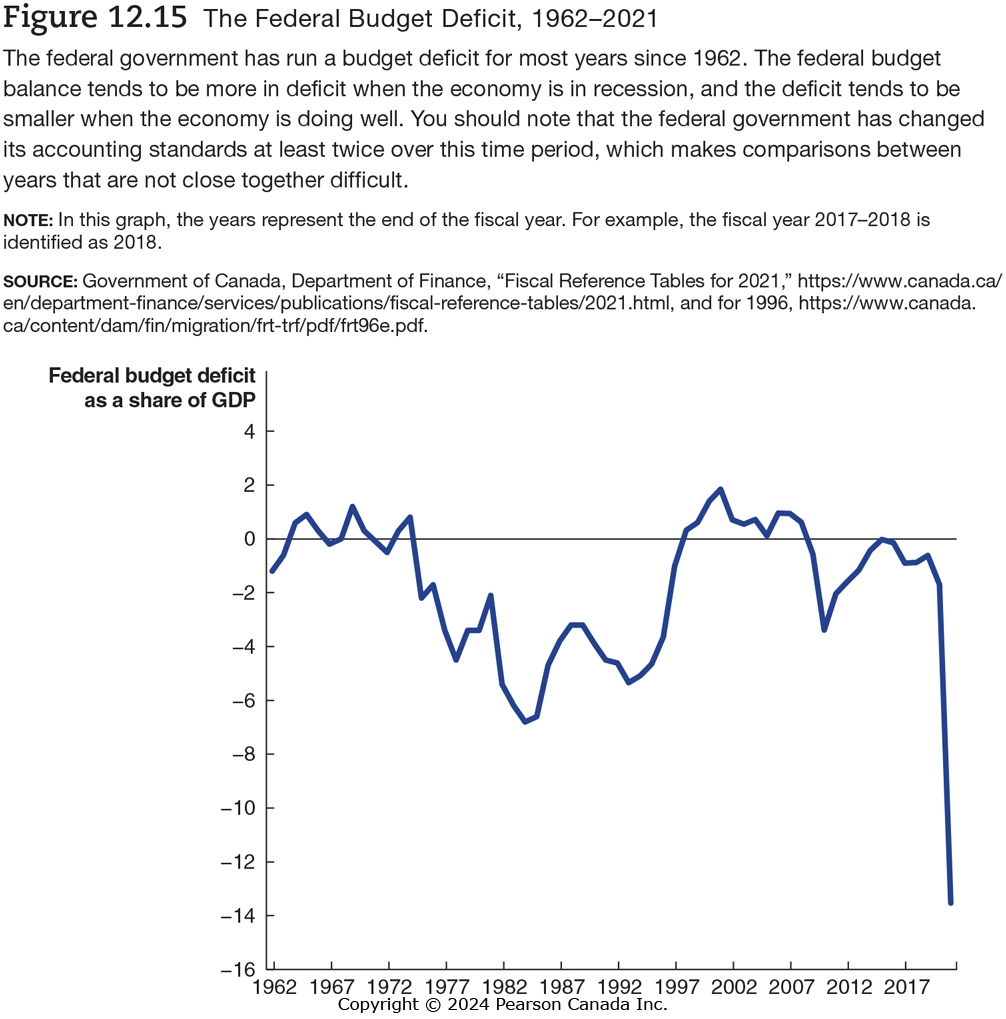
\includegraphics[width=0.48\linewidth]{Fig12-015}
\end{frame}

\begin{frame}{Deficits Over the Business Cycle}
\transfade
\begin{itemize}
  \item The federal government has run deficits in most years since the 1960s.
  \item Deficits tend to be \textbf{larger in recessions}:
  \begin{itemize}
    \item tax revenues fall as incomes and profits decline,
    \item automatic stabilizers like EI and welfare spending rise.
  \end{itemize}
  \item These automatic stabilizers help:
  \begin{itemize}
    \item limit the severity of recessions,
    \item partially offset declines in private demand.
  \end{itemize}
\end{itemize}
\end{frame}

\begin{frame}{Federal Government Debt}
\transfade
\begin{itemize}
  \item When the federal government runs a deficit, it finances this by selling \textbf{bonds}.
  \item The total value of outstanding federal government bonds is:
  \begin{block}{Federal government debt (national debt)}
    The total value of government securities outstanding.
  \end{block}
\end{itemize}
\end{frame}

\begin{frame}{Figure 12.16 -- Federal Government Debt, 1962--2021 }
\centering
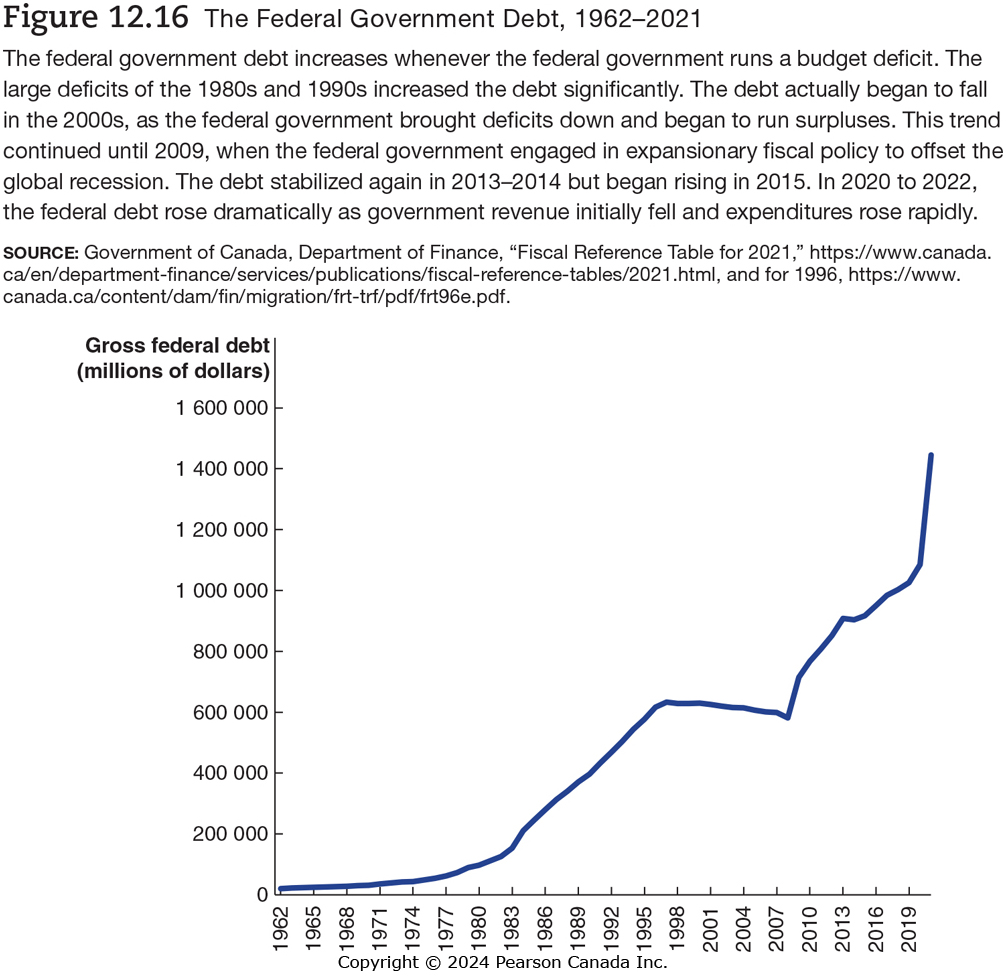
\includegraphics[width=0.47\linewidth]{Fig12-016}
\end{frame}

\begin{frame}{Is Government Debt a Problem?}
\transfade
\begin{itemize}
  \item Currently, the federal government faces no serious risk of default because:
  \begin{itemize}
    \item it can borrow at relatively low interest rates,
    \item interest payments are small relative to the overall budget.
  \end{itemize}
  \item In the \textbf{long run}, a debt that grows faster than GDP can be problematic:
  \begin{itemize}
    \item it may crowd out private investment,
    \item slowing long-run economic growth.
  \end{itemize}
  \item The concern is smaller if the debt finances \emph{productive} spending:
  \begin{itemize}
    \item infrastructure, education, research and development,
    \item which raise future potential GDP.
  \end{itemize}
\end{itemize}
\end{frame}

% ============================================================
\section{12.7 Fiscal Policy in the Long Run}
% ============================================================

\begin{frame}{12.7 Learning Objective}
\transfade
\begin{block}{Goal}
Discuss the effects of fiscal policy in the long run.
\end{block}
\begin{itemize}
  \item So far, we focused on short-run stabilization (AD).
  \item Now we consider long-run impacts on potential GDP (AS) via taxes and incentives.
\end{itemize}
\end{frame}

\begin{frame}{Supply-Side Economics}
\transfade
\begin{itemize}
  \item Some fiscal policy actions aim at long-run increases in potential GDP:
  \begin{itemize}
    \item these affect \textbf{aggregate supply}, not just aggregate demand.
  \end{itemize}
  \item Policies that focus on incentives to work, save, invest, and innovate are often called:
  \begin{block}{Supply-side economics}
    Fiscal policy aimed at increasing long-run aggregate supply, usually by changing taxes or regulations.
  \end{block}
\end{itemize}
\end{frame}

\begin{frame}{Tax Wedge and Marginal Tax Rates}
\transfade
\begin{itemize}
  \item Most taxes are assessed as a percentage of economic activity:
  \begin{itemize}
    \item individual income, corporate profits, capital gains, etc.
  \end{itemize}
  \item When an individual decides how much to work, they care about the:
  \begin{itemize}
    \item \textbf{post-tax wage}: how much an extra hour of work increases their consumption possibilities.
  \end{itemize}
  \item A firm deciding how many workers to hire cares about:
  \begin{itemize}
    \item the \textbf{pre-tax wage}: the total cost of employing each worker.
  \end{itemize}
  \item The difference between pre-tax and post-tax returns is known as the:
  \begin{block}{Tax wedge}
    The gap between the pre-tax and post-tax return to an economic activity, implied by the \emph{marginal tax rate}.
  \end{block}
\end{itemize}
\end{frame}

\begin{frame}{Why Tax Rates Matter}
\transfade
\begin{itemize}
  \item The larger the tax wedge, the stronger the behavioural response:
  \begin{itemize}
    \item individuals and firms have weaker incentives to engage in taxed activities.
  \end{itemize}
  \item Examples:
  \begin{itemize}
    \item \textbf{Individual income tax}:
      \begin{itemize}
        \item affects labour supply decisions and entrepreneurship.
      \end{itemize}
    \item \textbf{Corporate income tax}:
      \begin{itemize}
        \item affects incentives to undertake investment projects.
      \end{itemize}
    \item \textbf{Taxes on dividends and capital gains}:
      \begin{itemize}
        \item affect the supply of loanable funds,
        \item influence the real interest rate and firms’ financing decisions.
      \end{itemize}
  \end{itemize}
\end{itemize}
\end{frame}

\begin{frame}{Figure 12.17 -- Supply-Side Effects of a Tax Change}
\centering
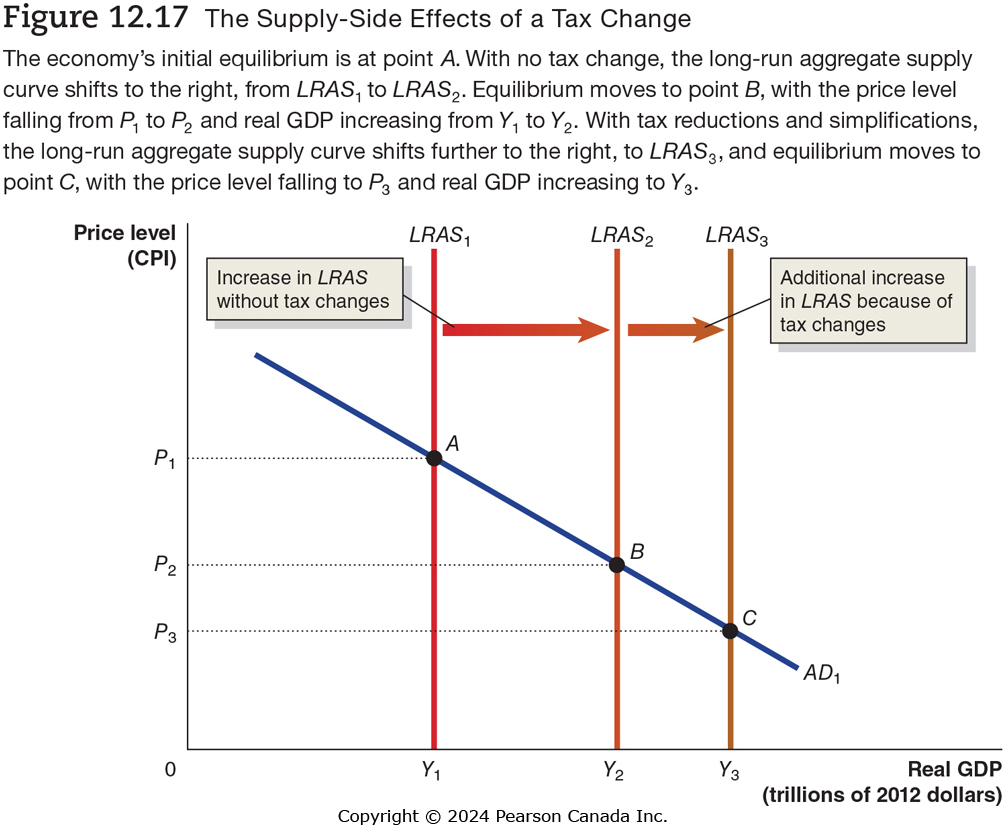
\includegraphics[width=0.57\linewidth]{Fig12-017}
\end{frame}

\begin{frame}{Long-Run Effects of Tax Reform}
\transfade
\begin{itemize}
  \item Tax reform has the potential to increase real GDP in the long run:
  \begin{itemize}
    \item by increasing work effort,
    \item by raising saving and investment,
    \item by encouraging entrepreneurship and innovation.
  \end{itemize}
  \item But the \textbf{magnitude} of these effects is uncertain:
  \begin{itemize}
    \item people may want to work more at lower tax rates,
    \item but may be constrained by employer expectations (e.g. a standard 40-hour week).
  \end{itemize}
  \item Economists agree that more research is needed on the quantitative impact of tax reforms.
\end{itemize}
\end{frame}

% ============================================================
\section*{Appendix: A Closer Look at the Multiplier}
% ============================================================

\begin{frame}{Appendix -- Learning Objective}
\transfade
\begin{block}{Goal}
Apply the multiplier formula using a simple macroeconomic model.
\end{block}
\begin{itemize}
  \item Build a simple model of how real GDP is determined.
  \item Derive:
  \begin{itemize}
    \item the government purchases multiplier,
    \item the tax multiplier,
    \item and the “balanced-budget” multiplier.
  \end{itemize}
\end{itemize}
\end{frame}

\begin{frame}{An Expression for Equilibrium Real GDP (1 of 2)}
\transfade
\begin{itemize}
  \item For simplicity, initially assume:
  \begin{itemize}
    \item taxes do not depend on income (fixed amount),
    \item there are no government transfers to households,
    \item there are no imports or exports (closed economy),
    \item the price level is constant.
  \end{itemize}
  \item Consider the following system (numbers in billions):
\end{itemize}
\begin{center}
\small
\begin{tabular}{p{0.44\linewidth} p{0.42\linewidth}}
\toprule
\textbf{Equation} & \textbf{Interpretation} \\
\midrule
1. \( C = 1{,}000 + 0.8(Y - T) \) & Consumption function \\
2. \( I = 125 \) & Planned investment function \\
3. \( G = 125 \) & Government purchases function \\
4. \( T = 100 \) & Tax function \\
5. \( Y = C + I + G \) & Equilibrium condition \\
\bottomrule
\end{tabular}
\end{center}
\end{frame}

\begin{frame}{An Expression for Equilibrium Real GDP (2 of 2)}
\transfade
\begin{itemize}
  \item These numbers are in billions of dollars.
  \item Consumption depends on disposable income \(Y - T\).
  \item Substituting into the equilibrium condition \(Y = C + I + G\), the slides write:
  \[
    Y = 100 + 0.8(Y - 100) + 125 + 125
  \]
  \item Subtracting \(0.8Y\) from both sides and simplifying leads to an equilibrium value of real GDP of approximately \(\$13\) trillion in this example.
  \item The exact numbers are less important than the \textbf{method}:
  \begin{itemize}
    \item substitute behavioural equations into the equilibrium condition,
    \item solve for \(Y\).
  \end{itemize}
\end{itemize}
\end{frame}

\begin{frame}{Algebraic Expression for Equilibrium Real GDP}
\transfade
\begin{itemize}
  \item Instead of plugging in numbers, we can work algebraically.
  \item Let:
  \[
    C = \bar{C} + \text{MPC}\,(Y - T), \quad
    I = \bar{I}, \quad
    G = \bar{G}, \quad
    T = \bar{T}
  \]
  \item The equilibrium condition:
  \[
    Y = C + I + G
  \]
  becomes:
  \[
    Y = \bar{C} + \text{MPC}(Y - \bar{T}) + \bar{I} + \bar{G}.
  \]
  \item Collect terms in \(Y\) to solve for equilibrium real GDP in terms of the autonomous components.
\end{itemize}
\end{frame}

\begin{frame}{Government Purchases Multiplier}
\transfade
\begin{itemize}
  \item Any change in an autonomous variable changes equilibrium \(Y\).
  \item Write the equilibrium condition in \emph{change} form (using \(\Delta\)):
  \[
    \Delta Y = \text{MPC} \,\Delta Y + \Delta G + \Delta I + \Delta C_{\text{aut}} - \text{MPC}\,\Delta T
  \]
  \item Holding \(\Delta C_{\text{aut}} = 0\), \(\Delta T = 0\), and \(\Delta I = 0\), we get:
  \[
    \Delta Y = \text{MPC} \,\Delta Y + \Delta G.
  \]
  \item Rearranging:
  \[
    \Delta Y (1 - \text{MPC}) = \Delta G
    \quad \Rightarrow \quad
    \frac{\Delta Y}{\Delta G} = \frac{1}{1 - \text{MPC}}.
  \]
  \item This is the \textbf{government purchases multiplier}.
\end{itemize}
\end{frame}

\begin{frame}{Numerical Government Purchases Multiplier}
\transfade
\begin{itemize}
  \item Example: \(\text{MPC} = 0.8\).
  \item Then:
  \[
    \text{Government purchases multiplier}
      = \frac{1}{1 - 0.8} = \frac{1}{0.2} = 5.
  \]
  \item Interpretation:
  \begin{itemize}
    \item A \$10 billion increase in government purchases raises equilibrium real GDP by \(\$50\) billion in this simple model.
  \end{itemize}
\end{itemize}
\end{frame}

\begin{frame}{Tax Multiplier}
\transfade
\begin{itemize}
  \item Again, consider the change form, but now allow \(\Delta T \neq 0\) and hold \(\Delta G = \Delta I = \Delta C_{\text{aut}} = 0\):
  \[
    \Delta Y = \text{MPC} (\Delta Y - \Delta T).
  \]
  \item Rearranging:
  \[
    \Delta Y = \text{MPC} \,\Delta Y - \text{MPC} \,\Delta T
    \quad \Rightarrow \quad
    \Delta Y (1 - \text{MPC}) = - \text{MPC} \,\Delta T.
  \]
  \item So the \textbf{tax multiplier} is:
  \[
    \frac{\Delta Y}{\Delta T} = - \frac{\text{MPC}}{1 - \text{MPC}}.
  \]
  \item Example: if \(\text{MPC} = 0.8\),
  \[
    \frac{\Delta Y}{\Delta T} = -\frac{0.8}{0.2} = -4.
  \]
\end{itemize}
\end{frame}

\begin{frame}{Tax Multiplier: Numerical Example}
\transfade
\begin{itemize}
  \item With \(\text{MPC} = 0.8\):
  \begin{itemize}
    \item a \$10 billion \emph{increase} in taxes decreases real GDP by \(\$40\) billion,
    \item a \$10 billion \emph{cut} in taxes increases real GDP by \(\$40\) billion.
  \end{itemize}
  \item Note:
  \begin{itemize}
    \item the tax multiplier is \textbf{negative},
    \item and smaller in absolute value than the government purchases multiplier
          (4 vs. 5 in this example).
  \end{itemize}
\end{itemize}
\end{frame}

\begin{frame}{The Balanced Budget Multiplier}
\transfade
\begin{itemize}
  \item Suppose the government increases \(G\) and \(T\) by the \textbf{same} amount, say \$10 billion.
  \item The total effect on real GDP combines:
  \begin{itemize}
    \item the government purchases multiplier (\(+5\) in the example),
    \item and the tax multiplier (\(-4\) in the example).
  \end{itemize}
  \item Adding these:
  \[
    \Delta Y = (+5 - 4)\times 10\ \text{billion} = 1 \times 10\ \text{billion}.
  \]
  \item Therefore, the \textbf{balanced-budget multiplier} is:
  \[
    \frac{\Delta Y}{\Delta G} = 1
  \]
  when \(\Delta G = \Delta T\).
  \item Equal dollar increases in government spending and taxes lead to the same dollar increase in real GDP in the short run.
\end{itemize}
\end{frame}

% ============================================================
\section*{Chapter Summary}
% ============================================================

\begin{frame}{Summary}
\transfade
\begin{itemize}
  \item Fiscal policy refers to changes in federal taxes and purchases intended to achieve macroeconomic objectives.
  \item Expansionary fiscal policy (higher \(G\) or lower \(T\)) is used to close recessionary gaps;
        contractionary fiscal policy (lower \(G\) or higher \(T\)) is used to reduce inflationary pressures.
  \item Government purchases and tax changes have multiplied effects on real GDP
        through the induced changes in consumption.
  \item Fiscal stimulus faces timing problems and possible crowding out of private spending.
  \item The federal budget deficit and debt evolve with the business cycle and policy choices;
        debt is less problematic when it finances productive investment.
  \item In the long run, fiscal policy can affect potential GDP through supply-side channels,
        especially via tax rates and incentives.
  \item The multiplier framework helps quantify how changes in \(G\) and \(T\) affect equilibrium real GDP.
\end{itemize}
\end{frame}

\begin{frame}
\centering
\Huge \textbf{Thank you!}
\end{frame}

\end{document}
